\section{Resultados e Discussão}

Na checagem estática pós-calibração ha horizontal ($90°$ na Figura~\ref{fig:imagem2}), oito leituras consecutivas apresentaram $A_{cal,z} \text{ entre } +0,998 \text{ g e } +1,012 \text{ e}$, componentes horizontais próximas de zero ($A_{cal,x} \in [-0,030; -0,019] \text{ g; } A_{cal,y} \in [-0,027; -0,013] \text{ g}$) e normal |A| entre $0,999 \text{ g}$ e $1,012 \text{ g}$ (média $1,005 \text{ g}$), confirmando a remoção do offset de +$1,322 \text{ g}$ em \textbf{X}. Em seguida Validou-se o sistema de 10° a 140° (Tabela~\ref{tab:validacao} e Figura~\ref{fig:grafico}{}), consolidando o ponto de 30° pela média das aquisições realizadas. 


\begin{table}[htbp]
    \centering
    \caption{Validação Angular com Transferidor (N = 100 Leituras por Ponto)}
    \label{tab:validacao}
    
    \resizebox{\textwidth}{!}{%
    \begin{tabular}{c c c c}
        \toprule
        \textbf{Referência $\theta_{ref} \text{ [°]}$}              & 
        \textbf{Estimado $\theta_{med} \text{ [°]}$}                & 
        \textbf{Erro $e = \theta_{med} - \theta_{ref} \text{ [°]}$} & 
        \textbf{Desvio Padrão $\sigma \text{ [°]}$}                 \\
        \midrule
        
        10,00  & $20,862$  & $+10,862$ & $0,123$ \\
        30,00* & $40,659$  & $+10,659$ & $0,164$ \\
        50,00  & $55,574$  & $+5,574$  & $0,172$ \\
        80,00  & $78,007$  & $-1,993$  & $0,119$ \\
        90,00  & $88,141$  & $-1,859$  & $0,096$ \\
        100,00 & $97,248$  & $-2,752$  & $0,165$ \\
        120,00 & $112,918$ & $-7,082$  & $0,091$ \\
        140,00 & $130,503$ & $-9,497$  & $0,071$ \\
                
        \bottomrule
    \end{tabular}%
    }
    
    \vspace{0.2cm}
    
    \raggedright
    \footnotesize
    Fonte: Elaborado pelo autor (2026).
\end{table}

{\raggedright
\textit{\textbf{*}Média de duas aquisições em 30,00° ($43,143°$ com $\sigma = 0,096°$ e $38,174°$ com $\sigma = 0,232°$)}}

\begin{figure}[H]
    \centering
    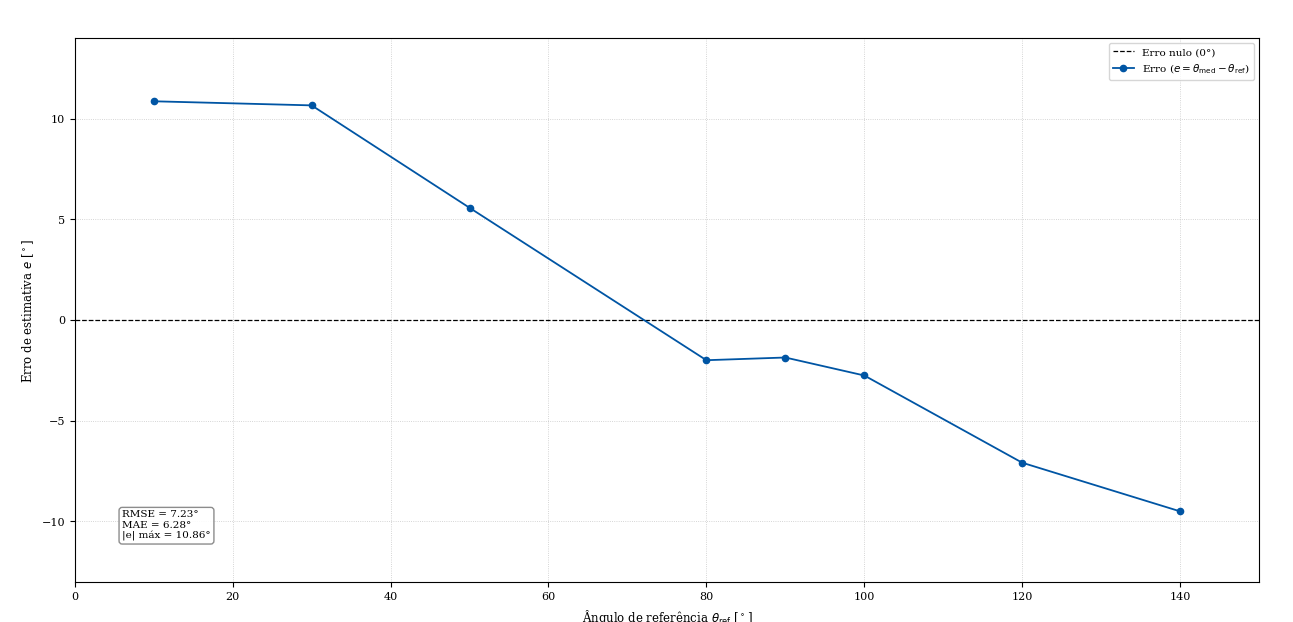
\includegraphics[width=1\linewidth]{IMG/Figure_1.png}
    \caption{Erro de estimativa ($e = \theta_{med} - \theta_{ref}$) versus ângulo de referencia (10° a 140°).}
    \label{fig:grafico}
\end{figure}


Nos oito pontos consolidados, obteve-se erro médio de $+0,489°$, MAE de $6,285°$, RMSE de $7,228°$ e erro máximo absoluto de $10,862°$ em $10°$ (ou RMSE = $7,74°$ e máximo de $13,143°$ considerando todas as nove leituras). Em contrates, a precisão eletrônica foi elevada em todas a faixa, com desvio padrão intra-ponto médio de apenas $0,129°$ (entre $0,071°$ e $0,232°$), demonstrando a eficiencia do filtro DLPF de 5 Hz e da promediação. A regressão linear entre $\theta_{med}$ e $\theta_{ref}$ resultou em $\theta_{med} = 0,830 \times \theta_{ref} + 13,70$ ($R^2 = 0,9989$),evidenciando que o erro não é aleatório, mas segue uma atenuação sistemática de $\approx 17\%$.

Esse padrão, positivo abaixo de $90°$, inferior a $2°$ próximo á horizontal acima de $90°$, decorre de fatores mecânicos e geométricos do aparato:

\begin{enumerate}
    \item \textbf{rigidez do chicote de jumpers}, que exerce torque restaurador nos ângulos extremos, puxando o bloco interno de volta ao centro;

    \item \textbf{folga residual no segundo eixo} do gimbal (refletida na dispersão de 4$,97°$ entre as duas leituras em $30°$);

    \item \textbf{erro de paralaxe visual} pela espessura da borda 3D sem ponteiro fino sobre o transferidor;

    \item \textbf{eventual desalinhamento entre o plano de giro e o plano XZ do chip}, projetando parte da gravidade em Y \cite{2.pedley2013}.
\end{enumerate}